%%%%%%%%%%%%%%%%%%%%%%%%%%%%%%%%%%%%%%%%%%%%%%%%%%%%%%%%%%%%%%%%%%%%%%
% Original Source: Dave Richeson (divisbyzero.com), Dickinson College
% Modified By: Chen Yiyang
% 
% A one-size-fits-all LaTeX cheat sheet. Kept to two pages, so it 
% can be printed (double-sided) on one piece of paper
% 
% Feel free to distribute this example, but please keep the referral
% to divisbyzero.com
% 
% Guidance on the use of the Overleaf logos can be found here:
% https://www.overleaf.com/for/partners/logos 
%%%%%%%%%%%%%%%%%%%%%%%%%%%%%%%%%%%%%%%%%%%%%%%%%%%%%%%%%%%%%%%%%%%%%%

\documentclass[10pt,landscape,letterpaper]{article}
\usepackage{amssymb}
\usepackage{amsmath}
\usepackage{amsthm}
\usepackage{physics} % for vectors
%\usepackage{fonts}
\usepackage{multicol,multirow}
\usepackage{spverbatim}
\usepackage{graphicx}
\usepackage{ifthen}
\usepackage[landscape]{geometry}
\usepackage[colorlinks=true,urlcolor=olgreen]{hyperref}
\usepackage{booktabs}
\usepackage{fontspec}
\setmainfont[Ligatures=TeX]{TeX Gyre Pagella}
\setsansfont{Fira Sans}
\setmonofont{Inconsolata}
\usepackage{unicode-math}
\setmathfont{TeX Gyre Pagella Math}
\usepackage{microtype}

\usepackage{empheq}

% new:
\def\MT@is@uni@comp#1\iffontchar#2\else#3\fi\relax{%
  \ifx\\#2\\\else\edef\MT@char{\iffontchar#2\fi}\fi
}
\makeatother

\ifthenelse{\lengthtest { \paperwidth = 11in}}
    { \geometry{margin=0.4in} }
	{\ifthenelse{ \lengthtest{ \paperwidth = 297mm}}
		{\geometry{top=1cm,left=1cm,right=1cm,bottom=1cm} }
		{\geometry{top=1cm,left=1cm,right=1cm,bottom=1cm} }
	}
\pagestyle{empty}
\makeatletter
\renewcommand{\section}{\@startsection{section}{1}{0mm}%
                                {-1ex plus -.5ex minus -.2ex}%
                                {0.5ex plus .2ex}%x
                                {\sffamily\large}}
\renewcommand{\subsection}{\@startsection{subsection}{2}{0mm}%
                                {-1explus -.5ex minus -.2ex}%
                                {0.5ex plus .2ex}%
                                {\sffamily\normalsize\itshape}}
\renewcommand{\subsubsection}{\@startsection{subsubsection}{3}{0mm}%
                                {-1ex plus -.5ex minus -.2ex}%
                                {1ex plus .2ex}%
                                {\normalfont\small\itshape}}
\makeatother
\setcounter{secnumdepth}{0}
\setlength{\parindent}{0pt}
\setlength{\parskip}{0pt plus 0.5ex}
% -----------------------------------------------------------------------

\usepackage{academicons}

\begin{document}

\definecolor{mathBlue}{cmyk}{1,.72,0,.38}
\definecolor{defOrange}{cmyk}{0, 0.5, 1, 0.3}
\definecolor{codeInlineRed}{cmyk}{0, 0.9, 0.9, 0.45}

\everymath{\color{mathBlue}}
\everydisplay{\color{mathBlue}}

% for vector notation in this module
\newcommand{\vect}[1]{\boldsymbol{#1}}
\newcommand{\deff}[1]{\textcolor{defOrange}{\textbf{#1}}}
\newcommand{\codein}[1]{\textcolor{codeInlineRed}{\texttt{#1}}}
\newcommand{\citeqn}[1]{\underline{\textit{#1}}}

\footnotesize
%\raggedright

\graphicspath{ {./img/} }

\begin{center}
  {\huge\sffamily\bfseries CS2106 Cheatsheet} \huge\bfseries\\
  by Yiyang, AY21/22
\end{center}
\setlength{\premulticols}{0pt}
\setlength{\postmulticols}{0pt}
\setlength{\multicolsep}{1pt}
\setlength{\columnsep}{1.8em}
\begin{multicols}{3}


% -----------------------------------------------------------------------
\section{Operating System Introduction}
\subsection{OS Overview}
\subsubsection{Terminology}
\deff{Multi-Programming} - The ability of the OS to run multiple programs, of same of different users, simultaneously.
\\
\deff{Time-Sharing} - The ability of the OS to support multiple users to interact with machine using terminals. Need Multi-programming.

\subsubsection{Common OS Structures}
\deff{Monolithic} - OS is a big, special program. The traditional approach taken by most Unix variants.
\\
\textbf{Pros}: 1) Ability to follow good SE principles, 2) Better Performance
\\
\textbf{Cons}: Highly coupled components and complicated internal structures

\medskip

\deff{Microkernel} - OS consists of many minimal kernels each providing basic and essential facilities, and microkernels are linked via IPC.
\\
\textbf{Pros}: 1) Simplicity, 2) More robust and extensible, 3) Better isolation \& protection
\textbf{Cons}: Communication across components take time, which penalises performance

\medskip

Other structures: \deff{Layered Systems}, \deff{Client-Server Model}.



\subsection{Hypervisor}
\deff{Hypervisors} \textasciitilde \ monitors ("containers") for running virtual machines, which allows other OS to run and debug on it. There are 2 types of Hypervisors
\begin{itemize}
    \item \deff{Type 1 \textasciitilde} - an OS working directly on hardware. Typically faster but more complicated. Expensive to acquire.
    \item \deff{Type 2 \textasciitilde} - a software (but not an OS) running in host OS. Simpler and can be used to emulate hardware you do not have.
\end{itemize}




\section{Process Management}
\subsection{Process}
A \deff{Process} is an abstraction to describe a running program. A \deff{Process Control Block} (PCB) (aka. \deff{Process Table Entry}) is a unit entity storing necessary information (\deff{Execution Context}) for a process. The \deff{Process Table} stores all  current PCBs.
\\
Context for a \textbf{Context Switch} includes: 1) Registers (GPR \& Special), 2) Stack Pointer, and 3) PC.

\subsubsection{Generic 5-State Process Model}
The Generic 5 States are: \deff{New}, 2) \deff{Ready}, 3) \deff{Terminated}, 4) \deff{Running}, and 5) \deff{Blocked}.
\\
\underline{Note:} Some systems (including Unix) do not have New - whenever a process is created, it is in Ready.

\medskip

In addition, in Unix, there are \deff{Orphan Process}, which is a child process with parent terminated before it, so the orphan is "adopted" by \codein{init} and waited properly when done, and 2) \deff{Zombie Process}, which is a child that has exited but the parent is executing but does not call wait on the child.

\subsection{Memory Regions}
The Memory consists of 1) \deff{Text} for instructions, 2) \deff{Data} for global variables, \deff{Heap} for dynamic allocation, e.g. via \codein{malloc()} in C, and 4) \deff{Stack} for function invocations.


\subsection{Stack \& Function Calls}
\subsubsection{Terminology}
In a function call, \deff{Caller} function invokes a function call of \deff{Callee}.
\\
A \deff{Stack Frame} stores information about one callee invocation, and there are two associated pointers. \deff{Stack Pointer} (SP) points to the top of the Stack while \deff{Frame Pointer} (FP) points to a fixed location in a Stack Frame.
\\
\underline{Note:} FP facilitates easy access of Stack Frame items. It is platform dependent and not compulsory. Every platform has SP.
\\
\deff{Register Spilling} is the practice of using memory to temporarily store GPRs' values so that GPRs can used reused for other purposes and restored afterwards. It is used during callee invocation.
\\
In a function call, \deff{Stack Frame Setup} is the preparation to make a function call, and \deff{Stack Frame Teardown} is the returning from function call.

\subsubsection{Stack Frame Setup and Teardown Example}
In \deff{Frame Setup}, \underline{Caller:} 1) Pass parameters with registers and/or stack, and 2) Save Return PC on stack; \underline{Callee:} 1) Save old SP, 2) Allocate space for local variables on stack, and 3) Adjust SP to point to new stack top.

\medskip

In \deff{Frame Teardown}, \underline{Callee:} 1) Place return result on stack (if applicable), and 2) Restore saved SP; \underline{Caller:} 1) Utilise return result (if applicable), and 2) Continue execution in caller following return PC.


\subsection{System Calls}
\deff{System Call} (aka. \deff{Syscall}) \textasciitilde \ API to OS, and it changes from User Mode to Kernel Mode (and changes back to User Mode after the syscall has completed). There are 3 ways of using Syscalls.
\begin{enumerate}
    \item Use the library version of the syscall. The library version serves as a \textbf{function wrapper} and typically has the same name. Applicable to most syscalls in modern languages.
    \item Use the user-friendly library version of the syscall. This version has related handles and serves as a \textbf{function adapter}. Few syscalls have such.
    \item Use the language's syscall method directly. E.g. in C, \codein{long syscall(long number, ...)}.
    
\end{enumerate}



\subsection{Exceptions, Traps \& Interrupts}
\deff{Exception} - Executing a machine level instruction can cause exceptions, e.g. arithmetic errors or memory accessing errors, and exception handlers are executed. Exceptions are \textbf{Synchronous}. 

\medskip

\deff{Trap} - Exceptions intentionally set-up. Trap is an easy-to-use mechanism to enter kernel mode. Aka. "software interrupts".

\medskip

\deff{Interrupt} - External events can cause interrupts during the execution of a program, as a form of notification, and interrupt handlers are executed. Interrupts are usually hardware-related and \textbf{Asynchronous}.



\section{Process Scheduling}
\subsection{Scheduling Overview}
Scheduling requires \deff{Scheduler}, the CPU component for process scheduling and \deff{Scheduling Algorithm}, that determines which process gets scheduled first.
\\
Depending on whether a process spends majority of time on CPU computation or I/O activity, it can be categorised as \deff{CPU Bound} or \deff{I/O Bound} activity.

\subsubsection{Types of Environment}
\begin{itemize}
    \item \deff{Batch Processing} - No user interaction or need to be responsive. Typically use non-preemptive scheduler since easier to implement.
    \item \deff{Interactive} - Involve user interaction and need to be responsive. Typically preemptive.
    \item \deff{Real-time} - All tasks have strict deadlines to meet and tasks are usually periodic.
\end{itemize}

\subsubsection{Types of Scheduling Policies}
\begin{itemize}
    \item \deff{Non-preemptive} - aka cooperative. A process stays scheduled until it blocks or gives up CPU voluntarily.
    \item \deff{Preemptive} - CPU can be taken from running process at any time.
\end{itemize}

\subsubsection{Scheduling Criteria}
All scheduling policies consider 1a) Fairness, whether it is biases against / towards any process, 1b) whether all processes can run without \deff{Starvation}, 2) Balanced utilisation of system resources, 3) \deff{Throughout}, number of tasks finished per unit time, 4) \deff{Turnaround Time}, total clock time taken (which is related to total/average waiting time), and 5) \deff{CPU Utilisation}, \% of time when CPU is working.
\\
In addition, Interactive System scheduling policies consider: 1) \deff{Response Time}, time between request and response by system, and 2) \deff{Predictability}, as it aims for less variance in response time.


\subsection{Batch Processing Scheduling Policies}
\subsubsection{First-Come First-Serve(FCFS)}
Maintain a Queue and add to Queue when new processes come. Run a task until it finishes or blocks, then choose next in Queue to run.
\\
\underline{Analysis:} Non-preemptive. No starvation. Sub-optimal avg waiting time.


\subsubsection{Shortest Job First (SJF)}
Maintain a Priority Queue of tasks to be scheduled, sorted in ascending order by the \textbf{estimated} CPU time needed for each task. 
\\
\underline{Analysis:} Non-preemptive. Starvation possible. CPU time can be estimated from the processes' past running time.

\subsubsection{Shortest Remaining Time (SRT)}
Preemptive version of SJF, where a new task can preempt currently running task if the estimated time for the former is less than remaining time needed for the latter.
\\
\underline{Analysis:} Preemptive. Starvation possible. Provide good service for short jobs.


\subsection{Interactive System Scheduling}
\subsubsection{Overview}
\deff{Time interrupt} is an interrupt that goes off periodically based on hardware clock and its handler invokes the scheduler to preempt a task. \deff{Interval of Time Interrupt} (ITI) is the timer period, i.e. smallest unit time in hardware clock for the timer. \deff{Time Quantum} is the execution duration given to a process, which can be constant or variable. It must be multiples of ITI.


\subsubsection{Round Robin (RR)}
Preemptive version of FCFS, where it runs the current task either until it blocks or gives up CPU, or when the time slice (\deff{quantum}) elapses. In the latter situation, put back the task to the rear of Queue.
\\
\underline{Analysis:} Preemptive, with a timer interrupt required. Response time guarantee, no starvation. Choice of quantum length affects performance.

\subsubsection{Priority Scheduling}
Maintain a Priority Queue and assign a priority value to every task to be scheduled. Choose tasks with highest priority every time. It can be preemptive or non-preemptive depending on whether higher priority tasks can preempt currently running tasks.
\\
\underline{Analysis:} Low priority tasks can starvation and preemptiveness does not help.


\subsubsection{Multi-Level Feedback Queue(MLFQ)}
Maintain multiple FIFO Queues of different priorities. Always pick from Queues of higher priority first, and run RR within each Queue. When a new task comes, put it in the highest priority Queue. Every time the tasks fully utilises its time slice, reduce its priority, otherwise retain its priority.
\\
\underline{Analysis:} Adaptive, seeking to minimise both response and turnaround time. Starvation possible. High priority Queues tend to have shorter time slices. Yet, possible to exploit the policy.


\subsubsection{Lottery Scheduling}
Scheduling is done rounds, where in each round, tasks are assigned "lottery tickets", the number of which depends on tasks' priority / estimate time. When picking a process to schedule, pick a ticket randomly from the pool then remove the task's tickets from the pool and pick from remaining tasks next time, until all tasks scheduled once for this round. New processes are not allowed to participate halfway during a round.
\\
\underline{Analysis:} Response time guarantee and no starvation. Good level of control. Simple.


\section{Inter-Process Communication}
\subsection{Common Mechanisms}
\subsubsection{Shared Memory}
Create a shared memory region once, and attach processes to the shared memory. All processes attached can read and write in shared memory just like to normal variables, achieving \textbf{implicit communication}. When done, detach all processes from the region and destroy it.
\\
\underline{Pros:} 1) Efficient, as no OS involvement during read and write to shared region, and 2) Ease of Use, as the implementation is simple and can be used for data of any type and size.
\\
\underline{Cons:} 1) Limited to a single machine, and 2) Synchronisation required as race conditions for shared variables can happen.


\subsubsection{Message Passing}
\textbf{Explicit} communication through exchange of messages. Process 1 prepares a message and send it to OS and Process 2 can receive it later. Both sending and receiving are syscalls.
\\
\underline{Pros:} 1) Safe, as guarded by OS, 2) Applicable beyond a single machines, 3) No need to synchronise.
\\
\underline{Cons:} 1) Inefficient, as all steps involve OS, 2) Hard to use, as data need to be packed/unpacked to supported message format.

\medskip

There are different variants of Message Passing, depending on its Naming Scheme and Synchronisation Behaviours.
\\
\deff{Naming Scheme} \textasciitilde \ How the sender/receiver identify one another
\begin{itemize}
    \item \deff{Direct Communication} - Send/Receiver explicitly names the other party. A form of 1-to-1 linkage. \underline{Pros:} Simple. \underline{Cons:} Impractical, especially since it requires the Receiver to know who sends it a message.
    \item \deff{Indirect Communication} - Messages are sent to / read from message storage (aka. \deff{Mailbox}), which can be shared among multiple processes. \underline{Pros:} Ability to have multiple senders and receivers.
\end{itemize}

\deff{Synchronisation Behaviour} \textasciitilde \ whether sending/receiving message is blocked until it is received/has arrived. For this module, assume \textbf{all receiving is blocked}.
\begin{itemize}
    \item \deff{Asynchronous MP} - Non-blocking Send. \underline{Pros:} Better flow for sender. \underline{Cons:} 1) Too much freedom for programmer, and 2) Not true asynchronous as \textbf{buffer size is finite}, so sending will block when buffer full.
    \item \deff{Synchronous MP} - Blocking Send, aka Rendezvous.
\end{itemize}
Synchronous MP can also be used as a form of synchronisation of two processes by using dummy message.



\subsection{Unix-Specific Mechanisms}
\subsubsection{Pipes}
In Unix, a process has 3 default communication channels, 1) \codein{stdin} for std input, 2) \codein{stdout} for std output, and 3) \codein{stderr} for std error output.

\medskip

Unix pipes behave like anonymous files, FIFO for data accessing order. Writer wait when pipe buffer is full, and reader waits when buffer empty. This enables Pipe to have \textbf{asynchronous} and \textbf{implicit} synchronisation.
\\
In addition there are \deff{half-duplex} (unidirectional) and \deff{full-duplex} (bidirectional) pipes.

\subsubsection{Signals}
\deff{Signals} are \textbf{asynchronous} (meaning can be sent anytime) notifications regarding an event, sent to a process/thread. The recipient must handle the signal by 1) a default set of handlers, or 2) user supplied handlers. \underline{Note:} Not all signal handlers can be override by user.
\\
Signals are sent from OS to user programs or from one user program to another. Signal handlers run in User Mode.
\\
With user supplied signal handlers, signals can achieve IPC.





\section{Threading}
\subsection{Threading Overview}
One process can have multiple threads, thereby achieving \deff{Data Parallelism} (different threads same task different data) and \deff{Task Parallelism} (different threads different tasks).
\\
\underline{Pros:} 1) Economy, as multi-threading easier than multi-processing, 2) Resource sharing, 3) Responsiveness, of multi-threaded programs, and 4) Scalability, as multi-threaded programs can utilise multiple cores / CPUs.
\\
\underline{Cons:} 1) Synchronisation getting more complicated, 2) Difficulty with \deff{System Call Concurrency}, and 3) Concerns regarding process behaviours (e.g. fork a multi-threaded process). 

\medskip

Certain information are shared across threads of the same process and some not shared.
\\
\underline{Shared:} 1) Text (code), 2) Data, 3) Heap, 4) File, and 5) Process ID.
\\
\underline{Not Shared:} 1) Thread Id, 2) Stack, 3) Registers (GPR \& Special), 4) PC



\subsection{Thread Implementation}
\subsubsection{User Thread}
\deff{User Thread} \textasciitilde \ Implemented as a user library. Not "recognised" or scheduled by the OS.
\\
\underline{Pros:} 1) Multi-threading can be done on any systems, 2) Context switch of threads easier, and 3) more configurable and flexible.
\\
\underline{Cons:} Sub-optimal performance with OS scheduling only processes.

\subsubsection{Kernel Thread}
\deff{Kernel Thread} \textasciitilde \ Implemented in OS, with thread operations handled as syscalls. Kernel schedules threads not processes.
\\
\underline{Pros:} Kernel can schedule threads.
\\
\underline{Cons:} 1) Slower and more resource-intensive with thread operations as syscalls, and 2) Generally less flexible.

\subsubsection{Hybrid Thread}
\deff{Hybrid Thread} \textasciitilde \ OS schedules only kernel threads while user threads can bind to kernel threads. More flexible.

% Illustration!


\section{Synchronisation}
\subsection{Critical Section}
\deff{Race Condition} - Interleaving of accesses to a shared modifiable resource. Race condition may lead to incorrect program behaviour so it is handled using \deff{Critical Section} (CS), which is designated code segment with race conditions. At any point of time, at most one process can be in the critical section.

\medskip

Critical Section has 4 properties:
\begin{enumerate}
    \item \deff{Mutual Exclusion} - If Process $P_1$ is in CS, all other processes are prevented from entering CS.
    \item \deff{Progress} - If no process is in a CS, one of the waiting processes should be granted access.
    \item \deff{Bounded Wait} - After Process $P_1$ requests to enter CS, there exists an upper bound on number of times other processes can enter CS before $P_1$.
    \item \deff{Independence} - Processes not executing in CS should never block (those waiting to enter CS).
\end{enumerate}
\underline{Note:} \#2 Progress requires \#4 Independence first, but it is possible to have \#4 Independence without \#2 Progress.
\\
\underline{Note:} \#2 Progress ensures no \deff{Deadlock}, a situation where all processes are blocked, and no \deff{Livelock}, a situation where all tasks are running but they do not "make any progress".


\subsection{HLL Implementation}
High-level Language (HLL) Implementations for Synchronisation are those using only normal programming constructs. (Use your brain power LOL)


\subsubsection{Failed Attempts}
\textbf{Attempt 1 - Lock Variable}: Use a shared boolean, \codein{lock}, to indicate whether any process in CS currently. Busy-wait if \codein{lock == 1}. Enter and update it if \codein{lock == 0}.
\\
\underline{Analysis:} \textbf{NOT WORK} as there can be race condition on \codein{lock} as well, violating \# 1 Mutual Exclusion.

\medskip

\textbf{Attempt 2 - Disable Interrupt}: As a fix to Attempt 1, disable interrupt (and hence no context switching) before a process waits or enters CS, and re-enable interrupts after it leaves CS.
\\
\underline{Analysis:} \textbf{NOT RECOMMENDED} as it only works on single-core systems and there can be race conditions with processes running on other cores in multi-core systems. In addition, disabling interrupts requires permission and is dangerous.

\medskip

\textbf{Attempt 3 - Turn Variable}: Use a shared variable, \codein{turn}, to indicate which process' turn it is currently. A process checks turn variable and waits until it is its own turn to enter CS.
\\
\underline{Analysis:} \textbf{NOT WORK} as it may violate \#4 Independence (\codein{turn = 0} and $P_1$ busy-waits but $P_0$ never enters CS).

\medskip

\textbf{Attempt 4 - Want Variable}: Use a shared boolean array, \codein{want[]}, where each element \codein{want[i]} indicates if Process $P_i$ wants to enter. (In case of 2 processes,) enter if the other process does not want to enter, otherwise wait.
\\
\underline{Analysis:} \textbf{NOT WORK} as it can have a deadlock when \codein{want[0] == 1} and \codein{want[1] == 1}, thereby violating \#2 Progress.


\subsubsection{Synchronisation Algorithms}
\deff{Peterson's Algorithm} - Combine Attempt 3 and 4. (In case of 2 processes,) wait if the other is waiting and it is the other's turn. If it is my turn, I will enter regardless.
\\
\underline{Analysis:} \textbf{WORK}, but 1) difficult to generalise for $\geq 3$ processes, and 2) Busy waiting is used and it is not desired.


\subsection{Assembly Level Implementation}
\deff{Test-Set-Lock} (TSL) \textasciitilde \ Similar to HLL Attempt 1 Using Lock Variable, but TSL does not have race condition because it is an \deff{Atomic}, i.e. reading and writing of the variable can only be done by one process at any time, operation ensured by the hardware.
\\
\underline{Cons:} Busy waiting.


\subsection{HLL Abstraction}
\subsection{Semaphore}
\deff{Semaphore} - A generalised synchronisation mechanism with functional behaviour of wait and signal. 

\subsubsection{Implementation}
\begin{itemize}
    \item An integer \codein{S} \textasciitilde \ number of "net wake-ups". Can be initialised to any non-negative integer.
    \item \codein{wait(S)} - decrement \codein{S}, and if $S \leq 0$, (process calling the semaphore) blocks. Aka. \codein{P()} or \codein{down()}.
    \item \codein{signal(S)} - increment \codein{S}, and wait up one sleeping process if any. Aka. \codein{V()} or \codein{up()}.
\end{itemize}
\underline{Note:} Assume no negative value for semaphore in this module.

\subsubsection{Functionality}
A \deff{Binary Semaphore} that \textbf{initialises to 1} and \textbf{ensures only value 0 or 1} is a \deff{Mutex}, i.e. Mutual Exclusion, for preventing race conditions.
\\
\underline{Note:} Deadlock can be avoided but is possible with improper implementation of two or more mutexes.

\medskip

A \deff{General Semaphore} serves as a General Synchronisation Tool (not CS in this case) for multiple processes (e.g. ensuring Processes $P_1, P_2, P_3$ operate in a fixed order.
\underline{Note:} Semaphore do not use busy waiting.

\subsection{Others}
\deff{Conditional Variable} - An implementation that allows a task to wait for certain event to happen. It can \deff{broadcast}, which wakes up all waiting tasks.







\section{Classical Synchronisation Problems}
\subsection{Producer-Consumer Problem}
\underline{Specification:} Processes share a bounded buffer of size $K$. Producers produce items to insert in buffer when buffer not full. Consumers remove items from buffer when buffer is not empty.

\medskip

\textbf{Solution 1 - Busy Waiting}: Use two shared booleans \codein{canProduce} and \codein{canConsume} for indication. Busy wait on the two booleans. Use another semaphore mutex to ensure no race condition where one of production / consumption can take place at a single time (as both will affect count). \underline{Analysis:} Solve the problem but uses Busy Waiting, which is not desired.

\medskip

\textbf{Solution 2 - Blocking}: Use semaphores \codein{notFull} and \codein{notEmpty} to force producers and consumers that are “inappropriate” at the current time to go to sleep, and to wake them up when “appropriate”. \underline{Analysis:} Solve the problem efficiently.

\medskip

\textbf{Solution 3 - Message passing}: Use built-in message passing with desired mechanisms - block on read when empty, block on write when full.


\subsection{Reader-Writer Problem}
\underline{Specification:} Processes share a data structure $D$ where Readers can retrieve information from $D$ and Writers can modify information in $D$. Write must have exclusive access to $D$, while Reader can access with other Readers. i.e. Must write along but can read together.

\medskip

\underline{Solution:} Refer to the diagram for solution. Intuitively, it means when there is an existing writer, the first reader waits at the semaphore while subsequent ones wait at the mutex. \underline{Analysis:} Works, but starvation may arise (e.g. when one write / many readers “hogging” the room).


\subsection{Dining Philosopher Problem}
\underline{Specification:} (This is a toy problem.) 5 Philosophers seat around a table with 5 single chopstick placed between every pair of philosophers. When any philosopher wants to eat, he/she will take both chopsticks from left and right. Devise a deadlock-free and starve-free algorithm for philosophers to dine.

\medskip

\underline{Solution 1 - Limited Eater} \textasciitilde "Social Distancing", allow at most 4 to try to eat.

\medskip

\underline{Solution 2 - Tanenbaum Solution} \textasciitilde “Turn \& Want” for Mutex Implementation.

\section{Memory Abstraction}
% very brief



\section{Contiguous Memory Allocation}
\deff{Contiguous Memory Management} \textasciitilde Process must be in memory, as one piece, during whole execution. So each process owns one contiguous memory region.

\subsection{Memory Partition}
\deff{Fixed-Size Partition} - Physical memory is split into fixed number of partitions of equal size. A process will occupy one. This partition scheme has \deff{Internal Fragmentation} - If a process does not occupy the whole partition, the leftover space is wasted.
\\
\underline{Pros:} 1) Easy to manage, 2) Fast to allocate (identical free partitions, no need choosing).
\\
\underline{Cons:} Partition size need to be large enough to contain largest possible process but larger partition size worse internal fragmentation.

\medskip

\deff{Variable-Size Partition} - Partition is created based on the actual size of process. OS keep track of the occupied and free memory regions. This partition scheme has \deff{External Fragmentation} \textasciitilde free memory space ("holes") created with process operations.
\\
\underline{Pros:} Flexible and ensure no internal fragmentation.
\\
\underline{Cons:} 1) Need to maintain information about each partition,  2) Extra time to locate appropriate free region for allocation.
\\
\underline{Note:} External fragmentation can be handled via \deff{Merging}, merging adjacent free holes, and \deff{Compaction}, moving occupied partitions around to create bigger consolidated holes, but they should not be done frequently.

\subsection{Dynamic Partitioning Algorithms}
\subsubsection{Allocation Methods}
There are 3 allocations methods: 1) \deff{First-Fit} finding first large-enough hole, 2) \deff{Best-Fit} finding smallest large-enough hole, and 3) \deff{Worst-Fit} finding largest hole.

\subsubsection{Allocation Implementation}
\textbf{Linked-List Method} - OS maintains a linked list for partition information, where each nodes represents one partition, storing info. about free/occupied, starting address and length, and pointer to next element.

\medskip

\textbf{Multiple-Free-List Method} - OS keeps separate sets of lists, one set of lists for free holes and the other for occupied partitions. In a set, there are multiple lists of different hole sizes (powers of two).
\\
\underline{Analysis:} Fast allocation (by getting holes of desired size)

\medskip

\textbf{Buddy System} - (A more efficient version of Multiple-Free-List) Free block is split into half repeatedly to meet request size. The two halves form a pair of sibling blocks ("buddies"). When both buddy blocks are free, they are merged to former a larger block and checked with its own buddy. 
\\
\underline{Note:} {[1]}Two adjacent free blocks of same size cannot be merged if they are not buddy. {[2]} When there is no occupied partition, the physical memory is one single free block.




\section{Disjoint Memory Allocation}
\deff{Disjoint Memory Allocation} \textasciitilde Processes can have disjoint chunks of memory space allocated.

\subsection{Paging}
\deff{Paging} \textasciitilde The physical memory is split into regions of fixed size, known as \deff{Physical Frames} (with size determined by hardware). Logical memory \textbf{of a process} is also split into regions of the same size, known as \deff{Logical Pages}. \underline{Note:} Logical pages are continuous while physical frames are disjoint.
\\
\deff{Page Table}, a lookup take for translation between pages and frames \textbf{per process}, is used for bookkeeping. The physical address can be calculated:
\[
\text{Physical Addr } = \text{ Frame ID } \times \text{ size$($Frame$)$ } + \text{ Offset } 
\]
, where $\text{ Frame ID }$ is obtained from Page Table for each page and $\text{ Offset }$ is displacement from beginning of page.
\\
\underline{Analysis:} 1) Paging has no external fragmentation. 2) Paging has internal fragmentation but always less than 1 page per process.

\subsubsection{Implementation}
Paging scheme needs to keep track of page tables of processes efficiently. Below are two implementations.

\medskip

\textbf{Software Solution} - OS stores Page Table in PCB, and considers it part of memory context of a process.
\\
\underline{Analysis:} Slow, as each memory ref now requires 2 memory accesses (1 to read page table entry for Frame ID, 1 to access actual memory)

\medskip

\textbf{Hardware Solution} - OS has a special component, \deff{Translation Look-Aside Buffer} (TLB), to support paging. It is a cache for page table entries, one TLB per core. \codein{TLB-Hit} and \codein{TLB-Miss} refer to entry found / not found in TLB. Only when not found in TLB, retrieve from Page Table in memory and update TLB.

\subsubsection{Application}
\textbf{Protection} - Paging can be easily extended to provide memory protection for each entry in a Page Table, using \deff{Access-Right Bits} (\codein{wrx} in Linux) and \deff{Valid Bits}.

\medskip

\textbf{Sharing} - Page table can allow several processes to share the same physical memory frame by using same frame number. Example: share code (text) pages; implement Copy-On-Write between parent \& child.

\subsection{Segmentation}
\deff{Segmentation} \textasciitilde Memory is managed at the level of memory segments (Text, Data, Heap, Stack), each of which is mapped (disjointly) to a contiguous physical partition. 
\\
Each memory segment has 1) a name ( or a \codein{SegID}) and 2) a \codein{Limit}, indicating the exact range of the segment. A segment table stores segment entries for each process. Each logical address is represented \codein{<SegID, Offset>} and need to make sure $\text{Offset $<$ Limit}$ all the time.
\\
\underline{Pros:} Each segment is an independent contiguous memory space, so 1) Follow programmer's view of memory, easy to understand, 2) More Efficient bookkeeping, and 3) Segments can grow / shrink and be protected / shared independently.
\\
\underline{Cons:} Segmentation uses variable-size contiguous memory regions, so prone to external fragmentation.

\subsection{Segmentation with Paging}
\deff{Segmentation with Paging} \textasciitilde Each segment is now composed of several pages instead of a contiguous memory region. Each segment has a page table.
\\
\underline{Analysis:} 1) Perform no worse than Segmentation or Paging separately. 2) Able to handle different functionalities, as some metadata better managed at segment level and some page level.




\section{Virtual Memory Allocation}
\deff{Virtual Memory} \textasciitilde A continuation of the idea of Paging Scheme, while some pages are in physical memory, and more “pages” in secondary storage. A \codein{resident bit} in page table entry indicates whether a page is in physical memory.
\\
CPU can only access memory resident pages. A \deff{Page Fault} occurs when CPU tries to access a non-memory resident page. \deff{Thrashing} is when memory access results in page fault most of the time.

\medskip

Remedies / Attempted Solution for Thrashing:
\begin{itemize}
    \item \deff{Locality Principle}, both Temporal and Spatial
    \item Skewed Distribution of Object / Access Popularity
    \item \deff{Demand Paging}, where process starts with no memory-resident pages, and only allocate a page when there is a page fault.
\end{itemize}
Analysis of Demand Paging: \underline{Pros:} 1) Fast startup time for new process, and 2) Small "memory footprint". \underline{Cons:} 1) Process appears slow at the start due to multiple page faults, and 2) Page faults may have cascading effects on other processes.


\subsection{Page Table Structures}
\deff{Direct Paging} - Keep all entries in a single (page) table. The implementation used above. Requires the entire structure to be contiguous and fits in one page.
\\
\underline{Analysis:} It requires huge page table size for large (secondary) memory. Unrealistic.

\medskip

\deff{2-Level Paging} \textasciitilde Page the page table into smaller page tables, each with a "page table number". The first level "page table" is known as the \deff{Page Directory}, and it is stored in the Memory Context of each process in PCB.
\\
\underline{Pros:} 1) Bypass the requirement for entire structure to be contiguous in memory. 2) No need to allocate memory for empty blocks.
\\
\underline{Cons:} 1) Require 2 memory access to get the frame number. (Solution: Use \deff{MMU Caches}, "TLB for directory entries" to speed up page-table walk)

\medskip

\deff{Hierarchical Page Table} \textasciitilde Radix-tree structure that extends the idea of 2-Level Page Table to $n$-level. All tables are setup and wired by the OS in software, but traversed by hardware. Used in most modern computers.

\medskip

\deff{Inverted Page Table} - Keep a single mapping of physical frame to \codein{<pid, page\#>} that uniquely identifies a memory page. \underline{Note:} It stores pages belonging to all processes.
\\
\underline{Pros:} 1) Huge saving, one table for all processes. 2) Fast translation for answering "which process and page does this frame belong to?", an auxiliary structure.
\underline{Cons:} Slow translation from a process' page to physical frame.

\subsection{Page Replacement Algorithms}
\subsubsection{Page Replacement}
\deff{Eviction} is the freeing of a memory page to store information for a new memory page (e.g. bring in a non-memory resident page). When a \deff{Clean Page}, page not modified, is evicted, no need to write back. When a \deff{Dirty Page}, page modified, is evicted, need to write back.
\\
We want to find optimal page replacement algorithms so as to minimise page faults and access / updating of secondary memory.

\subsubsection{Algorithms}
\deff{Optimal Page Replacement} (OPT) - The theoretical optimal algorithm, not achievable but serves as a benchmark for comparison: If we have future knowledge of memory reference, replace the page that will not be needed again for the longest upcoming period, and this guarantees minimised page faults.

\medskip

\deff{FIFO Page Replacement} - Evict memory pages based on their loading time, i.e. evict the oldest memory page.
\\
\underline{Implementation:} OS maintains a queue for resident page numbers. Remove 1st in queue if replacement needed. Update queue during page fault trap.
\\
\underline{Pros:} Simple to implement, no need hardware.
\\
\underline{Cons:} 1) FIFO does not exploit temporal locality (, oldest memory $\neq$ not used recently). 2) Suffer from \deff{Belady's Anomaly}, where the number of physical frames increases, number of page faults should decrease intuitively, but in reality, more page faults occur for FIFO.

\medskip

\deff{Least Recently Used} (LRU) - Use the notion of temporal locality, and replace page not used in longest time. Aim to approximate OPT (predict future by mirroring the past).
\\
\underline{Pros:} Does not suffer from Belady's Anomaly.
\\
\underline{Cons:} Hard to implement and require additional hardware support.

\medskip

\deff{Second-Chance Page Replacement} (CLOCK) - Modified FIFO to give a second chance to pages that are accessed. 
\\
\underline{Implementation:} Use a \codein{Reference Bit} for each entry where \codein{1} for accessed since last reset and \codein{0} otherwise. For replacement, pop if ref bit \codein{0}, or reset the bit if \codein{1}. When access / bring in a page, update ref bit to \codein{1}. Use a Circular List.


\subsection{Frame Allocation}
\deff{Local Replacement} - Victim pages are selected among pages of the process with page fault. \underline{Pros:} Number of frames allocated to a process unchanged, so performance stable between multiple runs. \underline{Cons:} If frames allocated not enough, the process' performance affected.

\medskip

\deff{Global Replacement} - Victim pages can be chosen among all physical frames during a page fault. \underline{Pros:} Allow self-adjustment between processes. \underline{Cons:} 1) Badly behaved processes can affect others. 2) Number of frames allocated to a process different, so performance vary between runs.

\medskip

\deff{Working Set Model} helps determine number of frames allocated to each process. \deff{Working Set}, $W(t, \Delta)$ is the set of active pages in the time interval $(t - \Delta, t)$. It gives info. about frames needed.
\\
\underline{Analysis:} Accuracy of the model is affected by choice of $\Delta$: If too small, then may miss pages in current working set; If too big: then may contain pages in other working set.




\section{File System Abstraction}
\subsection{File System Introduction}
Criteria for a File System: 1) \textbf{Self-Contained}, able to "plug-and-play" on another system, 2) \textbf{Persistent}, beyond the lifetime of OS and processes, and 3) \textbf{Efficient}, which provides good management of free and used space, with minimal overhead.

\subsection{File}
A \deff{File} is a logic unit of info created by process. It contains \deff{Data} and \deff{Metadata}.
\\
Different FS have different naming rules, but they usually follow \codein{Name.Extension} format.

\subsubsection{File Type}
An OS commonly supports a number of file types, each with an associated set of operations and/or a specific program for processing it. Common file types:
\begin{itemize}
    \item \deff{Regular Files} - Files containing user info, and can be further categorised as \deff{ASCII Files}, can be displayed as it is, and \deff{Binary Files}, with a predefined internal structure to be processed by specific program.
    \item \deff{Directories} - System files for FS structure.
    \item \deff{Special Files} \textasciitilde character / block oriented.
\end{itemize}
To distinguish file types: 1) Use file extension as indication, or 2) Use embedded information in the file (e.g. \codein{Magic Number} at the beginning of a file in Unix)

\subsubsection{File Protection}
To control access to info stored in a file, restrict access based on user identity.
\begin{itemize}
    \item \deff{Access Control List} - Store a list of user identities and allowed access type. \underline{Pros:} Very customisable. \underline{Cons:} Additional info associated with file needed.
    \item \deff{Permission Bits} - Classify user into 3 classes (Owner, Group, Universe) and give \codein{wrx} bit for each class.
\end{itemize}

\subsubsection{File Data Structure \& Access Methods}
Structures how a file stores data
\begin{itemize}
    \item Array of Bytes: Each byte has a unique offset from file start. Hard to jump to any specific "entries".
    \item Fixed-Length Records: Can jump to any records.
    \item Variable-Length Records: Flexible but harder to locate a record.
\end{itemize}
Access Methods:
\begin{itemize}
    \item Sequential Access: Read data in order from file start. Cannot skip but can rewound.
    \item Ranom Access: Read data in any order. \codein{Read(Offset)} states the position to start access explicitly, or \codein{Seek()} to move to a new location in file. Both Unix and Windows FS use latter.
    \item Direct Access: i.e. random access to any records directly, used in files of fixed-length records.
\end{itemize}

\subsection{Directories}
\deff{Directories} provide a logical grouping of files (User view) and keep tracks of files (system usage).

\subsubsection{Links in Linux}
\deff{Hard Link} - Both files have separate pointers to the actual file in disk. Limited to only files.
\\
\underline{Pros:} Low overhead (only pointers added).
\\
\underline{Cons:} Deletion problem.

\medskip

\deff{Symbolic Link} - For $B$ being a symbol link of $A$ pointing to the actual file $F$, $B$ is a file $G$ with path name of $F$, so accessing $G$ means to find where $F$ is and access it. It acts as an "intermediate jump". Applicable to both files and directories.
\\
\underline{Pros:} Simple deletion: If $B$ deletes, $G$ gets deleted but $F$ unaffected. If $A$ deletes, $F$ is gone and $G$ remains but not working.
\\
\underline{Cons:} Large overhead, with special link file taking up actual disk space.


\subsubsection{Directory Structures}
\deff{Tree Structure} \textasciitilde Recursively embed directories in other directories, which forms a tree. To refer a file, use either absolute path-name from root directory, or relative path-name followed from current working directory.

\medskip

\deff{DAG Structure} \textasciitilde Based on the Tree structure, but a file can be shared in different directories. Only one copy of actual content exists but it appears in multiple directories of different path-names.
\\
In Linux, created with Hard Links.

\medskip

\deff{General Graph Structure} \textasciitilde Hard to traverse and maintain (determine when to remove a file / directory, prevention of infinite loops). Not desirable.
\\
In Linux, created with Symbolic Links.

\subsection{OS and File System}
OS provides syscalls for all file operations, and it also maintains information about FS.

\subsubsection{Runtime Information for Files}

Information kept for an opened file: 1) \deff{File pointer}, current location in file, 2) \deff{Disk Location}, actual file location on disk, and 3) \deff{Open Count}, number of processes that have this file opened.
\\
The OS also maintains a \deff{System-wide Open-File Table}, with one entry for each unique file opened, and \deff{Per-Process Open-File Table}, which has an entry for each file opened by the process, and the entry points to the one in the system-wide table. There is also \deff{Buffer} for information read from / written to disk.
\\
\underline{Implications:} Two processes can open the same file using same (e.g. parent \& child) or different file descriptors. Same process can also open one file twice simultaneously.

\subsubsection{File Operations}
To \codein{Create} a file: 1) Use full pathname to locate the parent directory. 2) Use free space list to find free disk blocks. 3) Add an entry to parent directory, with relevant file info \& metadata.

\medskip

To \codein{Open} a file $F$ in process $P$: 1) Search system-wide table for existing entry $E$: If found, create an entry in $P$’s table pointing to $E$; Otherwise, continue. 2) Use full pathname to locate file $F$: When $F$ is located, load its information into a new entry $E$ in system-wide table, and create an entry in $P$’s table pointing to $E$. 3) Return pointer to entry.




\section{File System Implementation}
\subsection{Hardware}
A \deff{Storage} is an 1D array of \deff{Logical Blocks}, smallest accessible units. Logical Blocks are mapped into disk sectors.
\\
Within one disk, there is a \deff{Master Boot Record} at Sector 0, which contains boot code and partition table. It is followed by several \deff{Partitions}, each containing an independent file system.
\\
Within one partition, there are 1) OS Boot-Up Information Block, 2) Block for Partition details (e.g. total number of blocks, number and location of free disk blocks), 3) Directory Structure, 4) Files' info., and 5) Actual File Data.


\subsection{File Implementations}
A file is implemented as a collection of logical blocks. There are different implementations, with different ways of 1) keeping track of the blocks, 2) allowing efficient access, and 3) utilising disk space effectively.

\medskip

\deff{Contiguous Allocation} - Allocate consecutive disk blocks to a file.
\\
\underline{Pros:} 1) Simple to keep track - Each file only needs starting block number \& length, 2) Fast access - only need to seek to first block.
\\
\underline{Cons:} 1) External fragmentation, 2) File size need to be specified in advance.

\medskip

\deff{Linked List Allocation} - Keep a linked list of disk blocks for each file. Each block stores 1) actual file data and 2) next disk block's number. File info stores first and last disk block number. 
\\
\underline{Pros:} No external fragmentation.
\\
\underline{Cons:} 1) Random access in a file is very slow. 2) Overhead for "pointers". 3) Less reliable (e.g. a pointer incorrect or a block corrupted.
\\
\underline{Variant:} Move all block pointers (of all files in the disk) into a single table, known as \deff{File Allocation Table} (FAT) and store FAT in memory during runtime. \underline{Pros:} Faster random access (memory traversal now). \underline{Cons:} FAT can be huge and consume valuable memory space.

\medskip

\deff{Indexed Allocation} -  Each file has an index block, an array that keeps track of (its) disk block addresses.
\\
\underline{Pros:} 1) Lesser memory overhead (than Linked List). 2) Fast direct access to certain location/offset of a file.
\\
\underline{Cons:} 1) Max file size limited by number of block entries in the index block. 2) Index block incurs overhead.
\\
\underline{Variant:} 1) \deff{Linked Scheme} - keeps a linked list of index blocks, can grow on demand. 2) \deff{Multi-Level Index Scheme} - Each first level index block points to several second level index blocks, with the last level being blocks for file data, example: Unix I-Node.


\subsection{Free Space Management}
\textbf{Bitmap Implementation} - Each disk block is represented by 1 bit (\codein{1} for free, \codein{0} for occupied). \underline{Pros:} Provide a good set of manipulations. \underline{Cons:} Need to keep the bitmap in memory for efficiency reason.

\medskip

\textbf{Linked List Implementation} - Use a linked list of disk blocks, where each disk block contains a number of free disk block numbers, and a pointer to next free space disk block. \underline{Pros:} 1) Easy to locate free blocks. 2) Only first pointer is needed in memory (though others can be cached). \underline{Cons:} High overhead.


\subsection{Directory Implementation}
A \deff{Directory Structure} keeps track of files in the directory and map file names to file information. Sub-directories are usually stored as file entries of special type. Several implementations for a Directory exists.
\begin{itemize}
    \item Linear List Implementation - A directory is a list, where each entry represents a file. Each entry stores 1) filename and metadata, and 2) file info / pointer to file info. Use linear search to locate a file. \underline{Analysis:} Linear search can be slow, so cache can be used to explore Locality as an improvement.
    \item Hash Table Implementation - Each directory has a hash table \codein{<FileName, File>}, and it uses Chained Collision Resolution. \underline{Analysis:} Fast lookup, but limited size for hash table and good hashing function is required.
\end{itemize}


\subsection{File Operation}
File operations are syscalls provided by the OS.



\subsection{Disk I/O Scheduling}
Time taken for one disk I/O is the sum of 1) \deff{Seek Time}, time for the disk head to move to a position over proper track, 2) \deff{Rotational Latency}, time for the desired sector to rotate under the I/O head, and 3) \deff{Transfer Time}, time to transfer data from disk sector to memory which depends on transfer size and transfer rate. 
\\
Time \#3 is negligible as compared to the other two (an order of 3 to 5). \textbf{Average time} of \#1 can be reduced with scheduling algorithms while Time of \#2 can be reduced with larger block size (at the compromise of \#3, but negligible).
\\
Scheduling Algorithms
\begin{itemize}
    \item FCFS - Simple but bad
    \item \deff{Shortest Seek First} (SSF) \textasciitilde SJF for disk context
    \item \deff{SCAN / Elevator Algorithm} \textasciitilde 1) bi-directional \deff{SCAN} that alternates between innermost and outermost, and 2) one-directional \deff{C-SCAN} that move from outermost to innermost (i.e. largest to smallest Track number)
\end{itemize}



\section{File System Case Studies}
\subsection{MS FAT}

\subsection{Linux Ext2}




\noindent\rule{8cm}{0.4pt}



\section{Intermediate Results \& Summary}
\subsection{From Tutorials}
\citeqn{(Tut1 Qn7)} In \codein{int *a = (int *) malloc(sizeof(int));}, the data, \codein{*a}, is created in the Heap while the pointer to this data, \codein{a}, can be in Stack or Data.

\citeqn{(Tut10 Qn3a)} When Process $A$ tries to open a file written by Process $B$, OS uses Open File Table to check for existing opened files and reject $A$'s request since the file is currently being written.

\citeqn{(Tut10 Qn3b)} When Process $A$ tries to use a bogus file descriptor for file-related syscalls, the OS checks whether the fd entry exists and is valid in $A$'s opened file table, and reject the syscall since invalid.

\citeqn{(Tut10 Qn3d)} Two processes $A$ and $B$ can read from the same file independently, as they have their own fds, which refers to two distinct locations in the open file table. Each entry of the open file table keep track of the current location separately. 

\subsection{From Past Questions}
\citeqn{(AY15/16Sem1 Midterm Qn1)} Library calls are language dependent, while syscalls depend only on the OS.

\medskip

\citeqn{(AY17/18Sem1 Midterm Qn8)} In scheduling, \textbf{Short Response Time} is not the same as \textbf{Bounded Waiting Time}. RR ensures latter but not former.

\medskip

\citeqn{(AY18/19Sem1 Final Qn8)} In Ext File System, data blocks for a file come from the same block group. One of the reasons is to reduce fragmentation.

\medskip

\citeqn{(AY18/19Sem1 Final Qn19)} In FAT File System, each Directory Entry is also stored in a logical block. So for file operations that modifies directory entry for the file, the logical block where the directory is in is also modified.

\medskip

\citeqn{(AY18/19Sem1 Final Qn25)} In Ext File System, \textbf{Disk Access Number} is the sum of accessing INodes and Contents starting from \codein{"/"}'s INode till the desired block in the file's content. (i.e. 2 accesses needed going down each directory level)




\subsection{Diagrams}
Onion Model of an Operating System:
\\
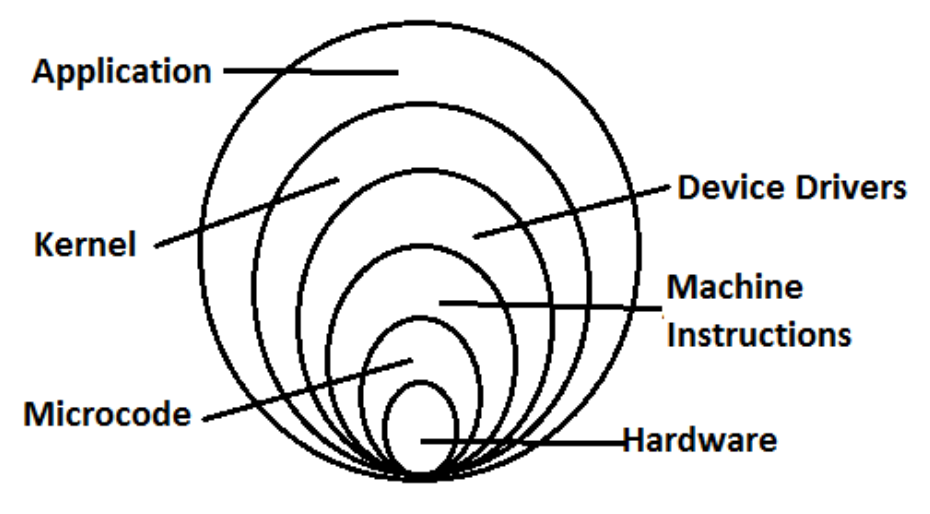
\includegraphics[width=8cm]{img/01_onion_model.png}

Generic 5 States of a Process:
\\
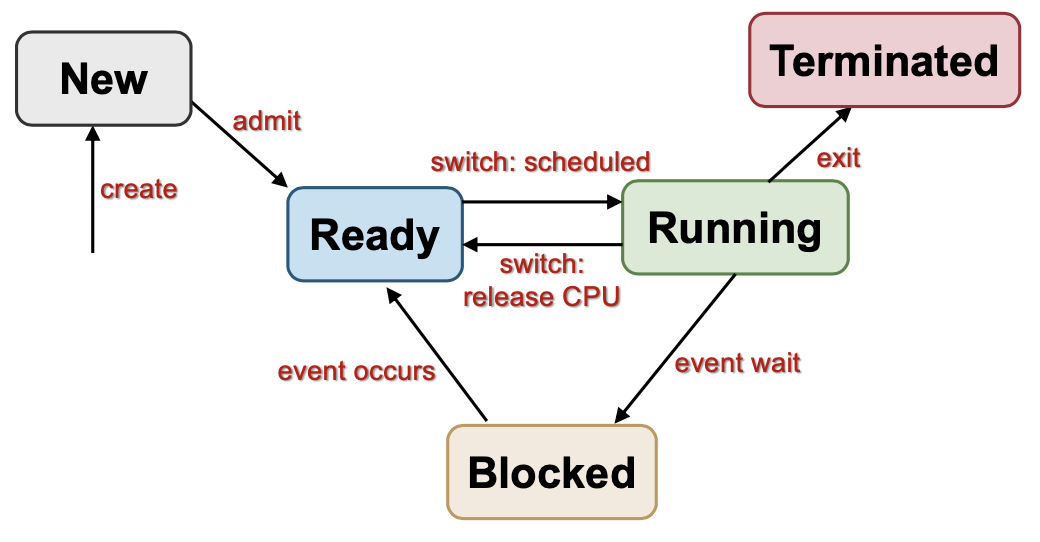
\includegraphics[width=8cm]{img/02_process_5_state.png}

Pseudocode for Peterson's Algorithm (note the order of updating variables before busy-wait):
\\
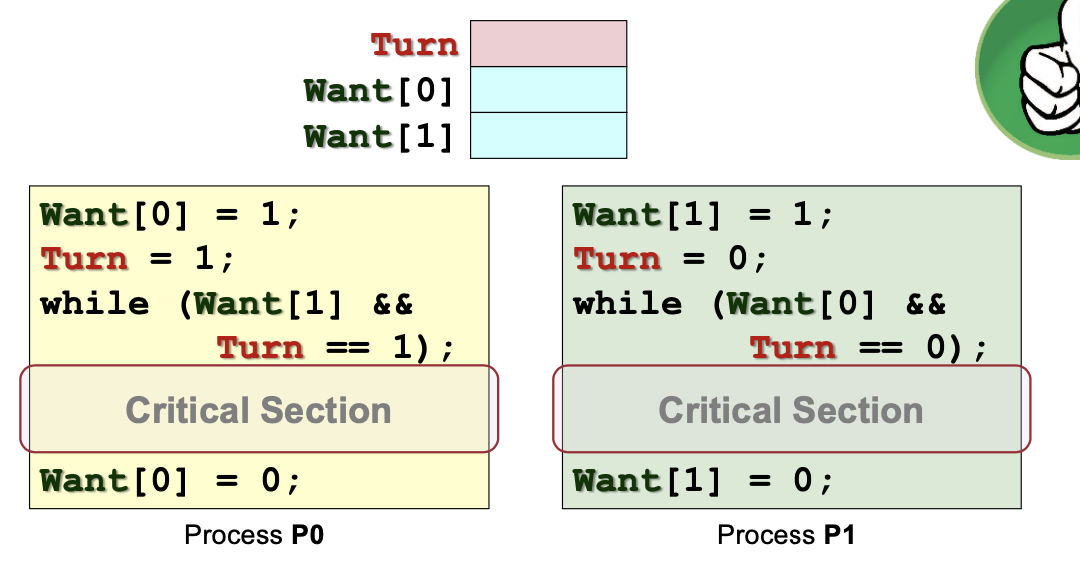
\includegraphics[width=8cm]{img/06_peterson.png}

Pseudocode for Solution to Reader Writer Problem:
\\
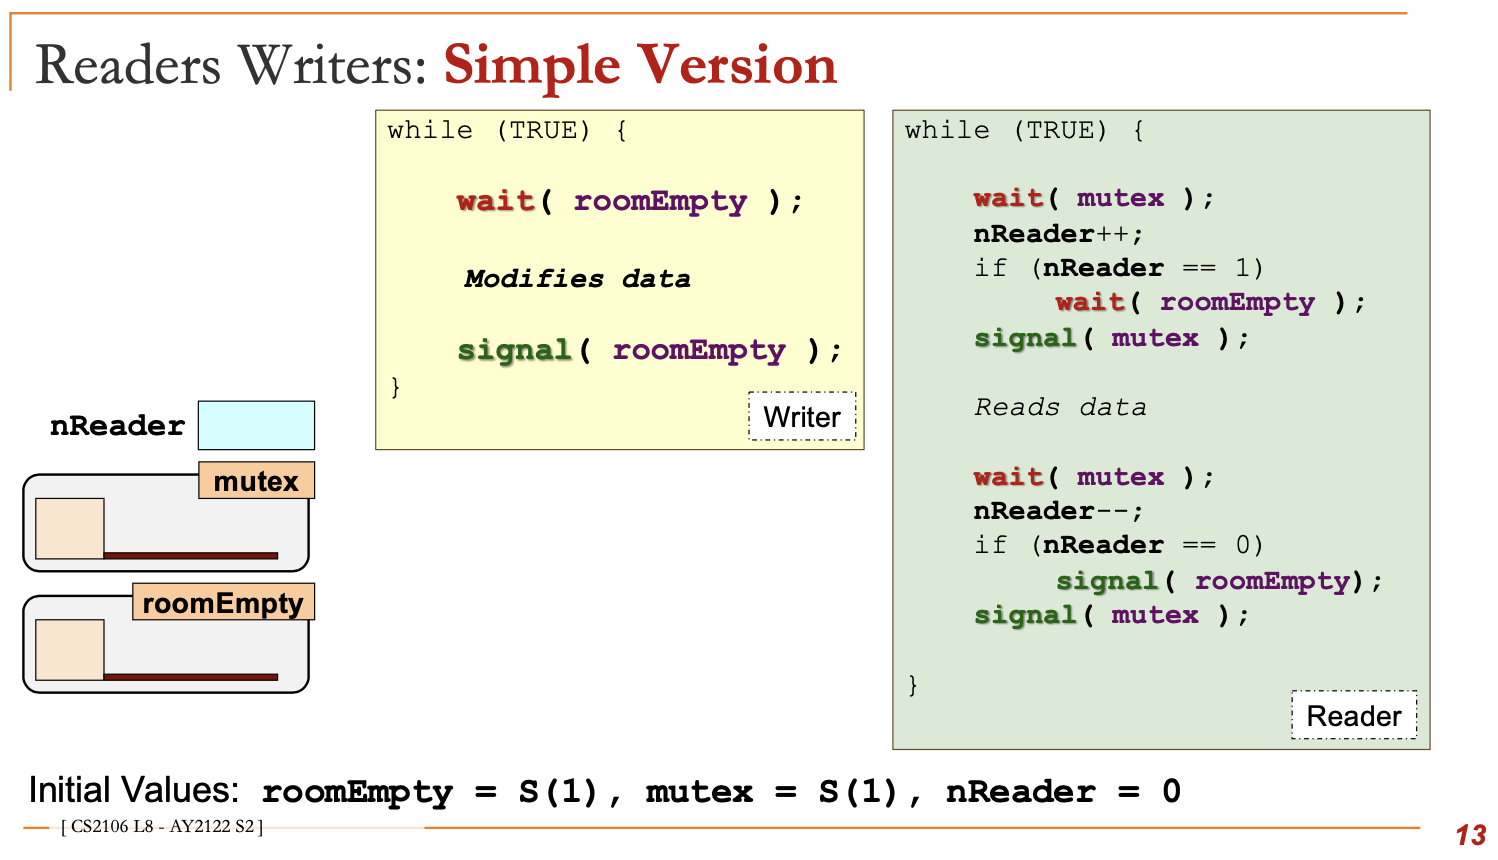
\includegraphics[width=8cm]{img/08_reader_writer.png}

Pseudocode for Tanenbaum Algorithm:
\\
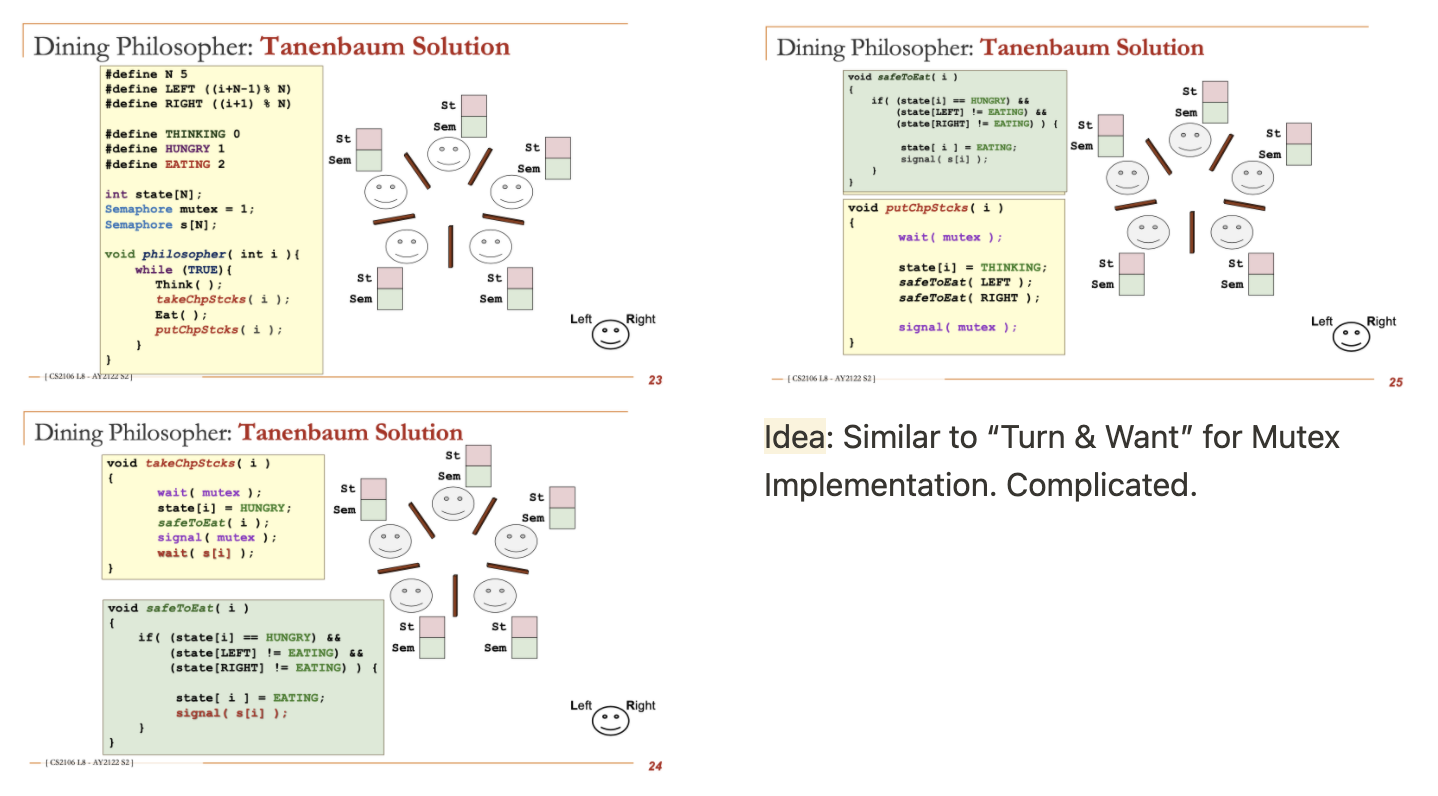
\includegraphics[width=8cm]{img/08_tanenbaum.png}

Illustration for Hiearchical Level Paging:
\\
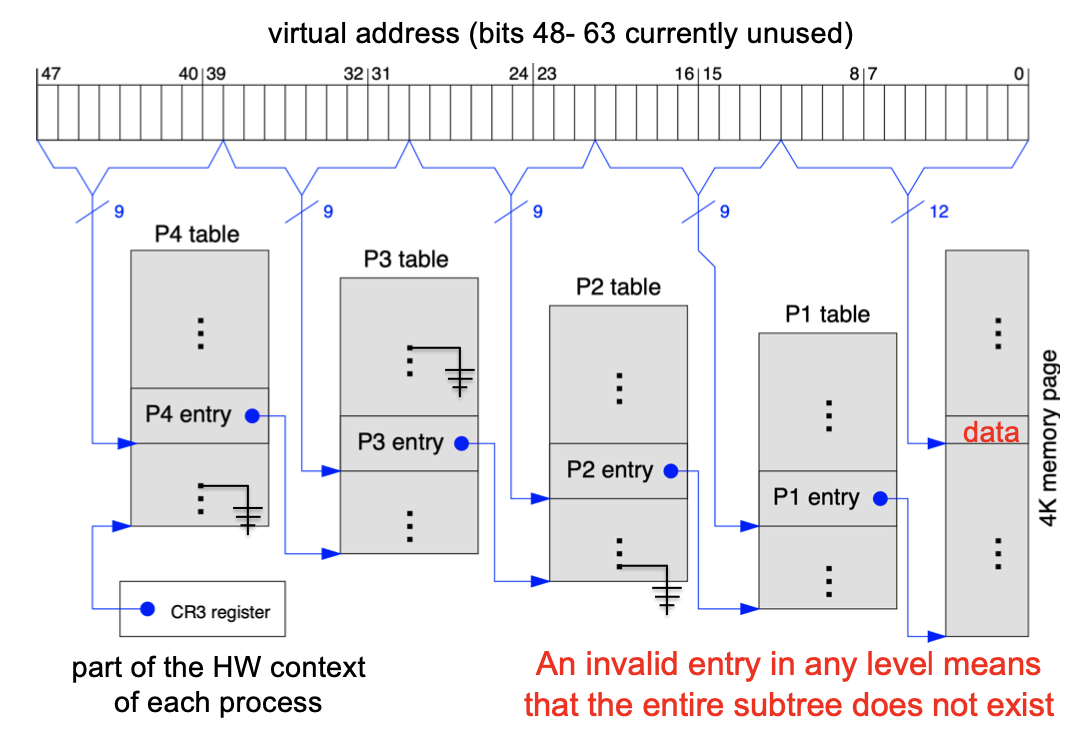
\includegraphics[width=8cm]{img/11_hierarchical_paging.png}

Illustration for File Opening:
\\
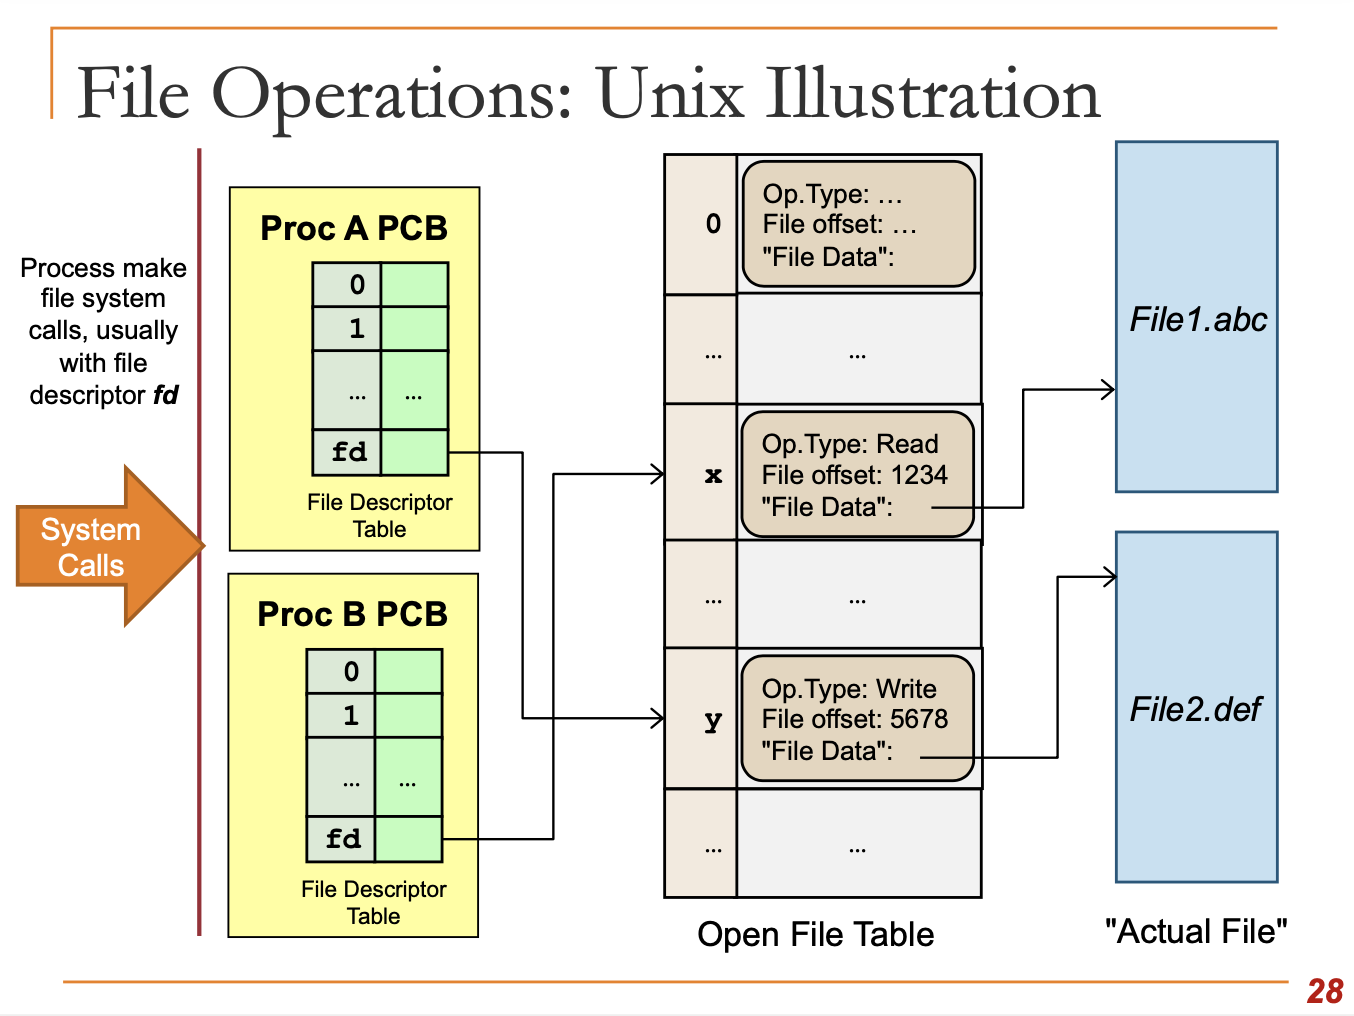
\includegraphics[width=8cm]{img/12_open_file_table.png}

Common File Operations:
\\
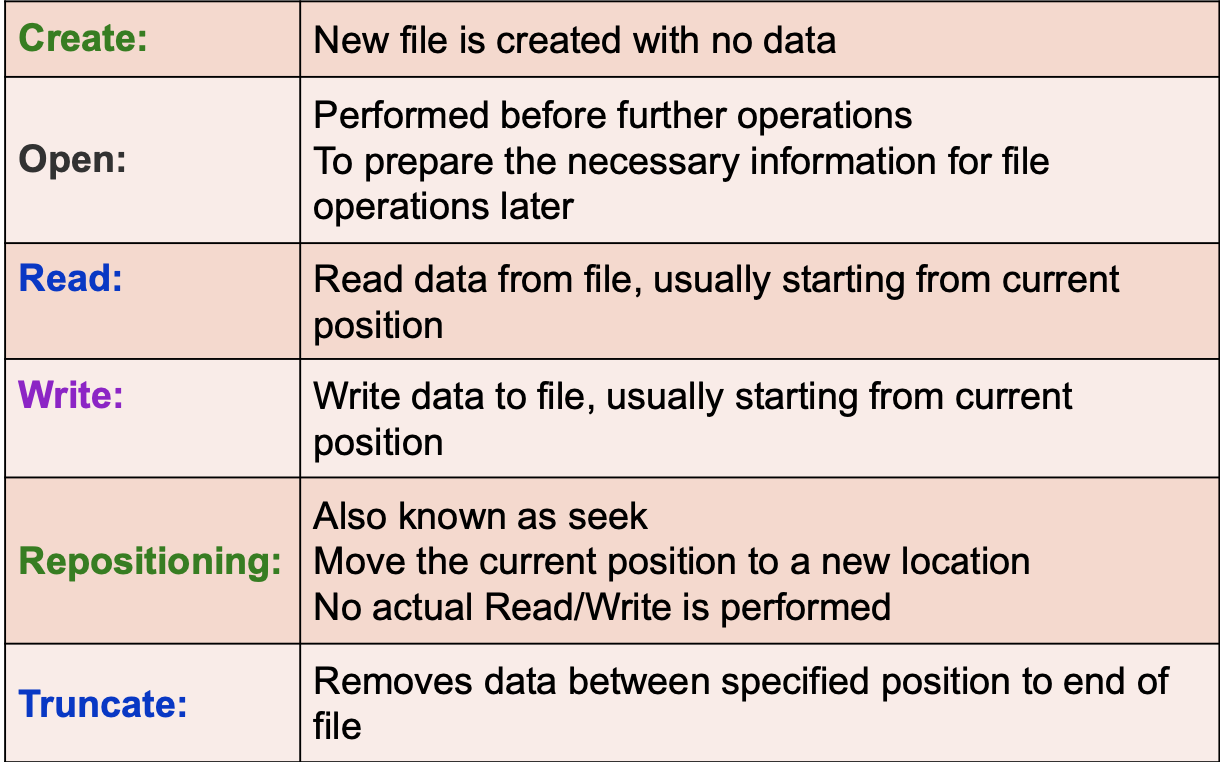
\includegraphics[width=8cm]{img/12_file_operations.png}

Illustration for One Slice of Magnetic Disk (note that multiple slices of disks stack over one another to form the hard disk):
\\
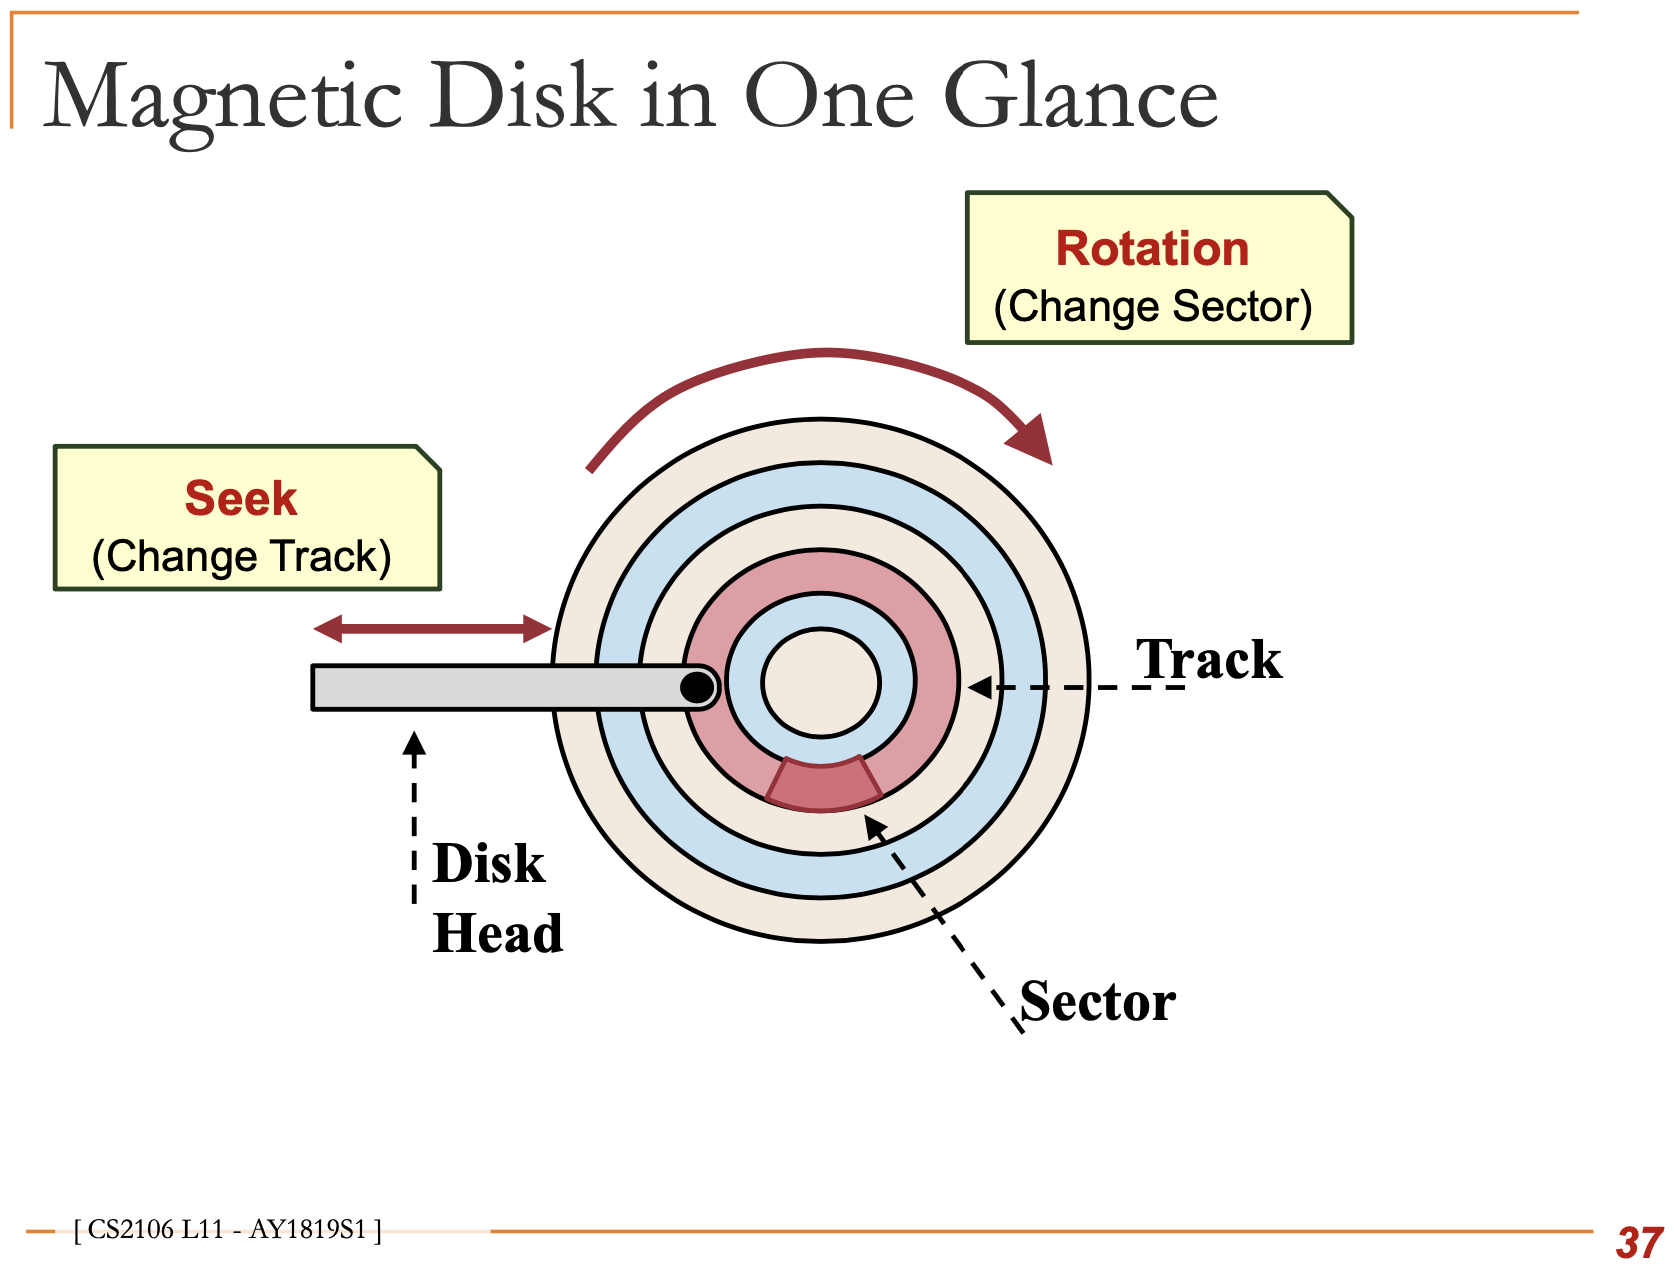
\includegraphics[width=8cm]{img/13_magnetic_disk_slice.png}

\citeqn{(Tut09 Qns3)} Algorithms for Virtual Memory Operations
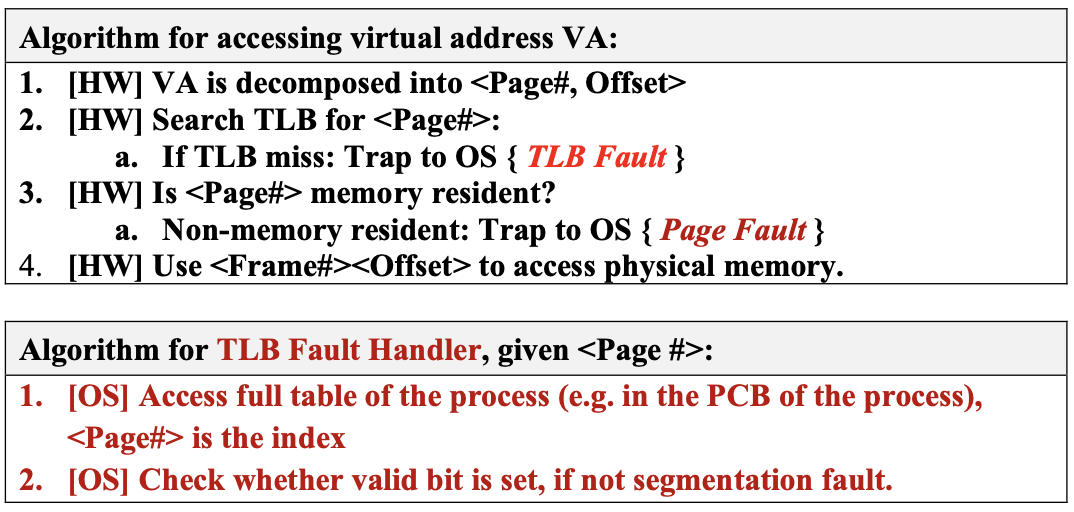
\includegraphics[width=8cm]{img/tut09_vm_algo_a.png}
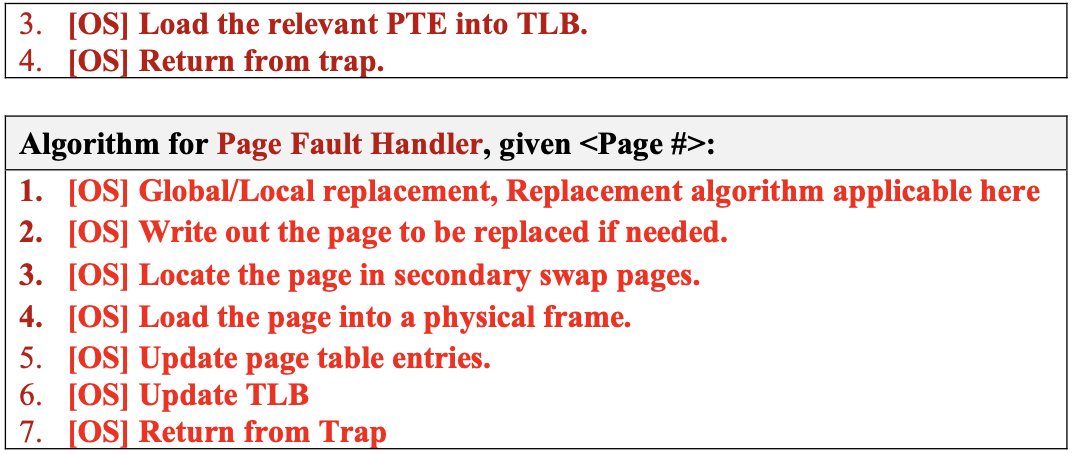
\includegraphics[width=8cm]{img/tut09_vm_algo_b.png}


\newpage




\section{Unix System Calls}
\subsection{Common Process Management Syscalls}
\subsubsection{\codein{fork()} Syscall}
\codein{int fork()} creates a duplicate of current process as a child process. It clones everything except PID and PPID. It returns the PID of child process forked in parent process and \codein{0} in child.
\\
Need header \codein{<unistd.h>}.


\subsubsection{\codein{exec*()} Family}
The family of syscalls, \codein{int exec*(...)}, replaces current executing process with a new one. It takes in path to the executable and arguments. It will not return when executing successfully and return \codein{-1} when fails.
\\
There are many variants, such as \codein{execv}, \codein{execl}, \codein{execle}, \codein{execlv}, or \codein{execv}, each with a slight difference in parameter specifications and behaviours.
\\
The typical usage is to create a new child process using \codein{fork()} then run the program using \codein{exec()} in the child.
\\
Need header \codein{<unistd.h>}.


\subsubsection{\codein{exit()} Syscall}
\codein{void exit(int status)} terminates the current process and the value of \codein{status} will return to the parent. The convention is \codein{0} for normal termination and non-zero for error.
\\
\codein{exit()} is the friendly wrapper of \codein{\_exit()} as the former does some necessary clean-up before invoking the syscall.
\\
When a child calls \codein{exit()}, it sends \codein{SIGCHLD} signal to the parent.
\\
Need header \codein{<unistd.h>}

\subsubsection{\codein{wait()} Family}
\codein{int wait(int *status)} makes the process block and wait for any one child process to terminate, and the exit status value is stored in the parent's variable referrenced by \codein{*status}. It cleans up remainder of terminated child's system resources.
\\
There are other variants such as \codein{waitpid()} that waits for a specific child.
\\
Need header \codein{<sys/types.h>} and \codein{<sys/wait.h>}.

\subsubsection{\codein{getpid()} Family}
\codein{int getpid()} returns the PID of the current process.
\\
There are similar syscalls such as \codein{getppid()}.
\\
Need header \codein{<unistd.h>}.



\subsection{IPC-Related Syscalls}
\subsubsection{\codein{pipe()} Syscall}
\codein{int pipe(int fd[2])} creates a unidirectional pipe channel with file descriptors \codein{fd[0]} for reading end and \codein{fd[1]} for writing end. It returns \codein{0} for successful creation and non-zero values for error.
\\
Need header \codein{<unistd.h>}.

\subsubsection{\codein{dup2()} Syscall}
\codein{int dup2(int oldfd, int newfd)} replaces the file descriptor of \codein{newfd} with the one specified by \codein{oldfd}.
\\
The syscall is typically used to redirect standard channels of a process to a pipe or file.
\\
Need header \codein{<unistd.h>}.



\subsubsection{Shared Memory Syscalls}
\codein{shmget()}, \codein{shmat()}, \codein{shmdt()}, and \codein{shmctl()} are syscalls to 1) create a shared memory region, 2) attach the shared memory to the current process, 3) detach the shared memory from the current process, and 4) destroy the shared memory region respective.
\\
\underline{Note:} \codein{shmget()} returns the ID of the shared memory created, and the ID is the identifier for the shared memory. A memory address is generated only when you attach a process to the shared memory using \codein{shmat()}. 
\\
Need header \codein{<sys/shm.h>}.


\subsection{Semaphore-Related Syscalls}
\codein{sem\_t} is the type for Semaphore. \codein{sem\_init()}, \codein{sem\_destroy()}, \codein{sem\_wait()}, and \codein{sem\_post()} are syscalls to 1) initialise a semaphore, 2) destroy the semaphore, 3) perform wait on the semaphore, and 4) perform signal on the semaphore respectively.
\\
Need header \codein{<semaphore>} and compile with option \codein{-lpthread}.







\end{multicols}
\end{document}
